\section{Clustering de semillas: Moreno-Dominguez.}

Moreno-Dominguez et al. \cite{Moreno-Dominguez2014} implementan el algoritmo
\textit{Agglomerative Hierarchical Clustering} para agrupar los tractogramas. 
En este algoritmo, cada \textit{feature} comienza en un cluster distinto. Luego,
el algoritmo selecciona iterativamente dos clusters siguiendo alg\'un criterio
de similitud; los agrupa en un nuevo cluster y crea un elemento representativo
de este. La jerarqu\'ia resultante de agrupar todos los clusters es expresada
como un dendrograma. En el trabajo de Moreno-Dominguez utilizan como medida de
similitud la distancia coseno (Ecuaci\'on \ref{eq:cosine}) y como criterio de
\textit{linkage} el centroide (Ecuaci\'on \ref{eq:centroide}).

\begin{figure}[h!]
                                                                                                                        
\begin{minipage}[b]{0.49\textwidth}
    \begin{equation}
        \label{eq:cosine}
        simil_{cos}(X,Y) = 1 - \frac{ X \cdot Y }{||X|| ||Y||}
    \end{equation}
\end{minipage} ~
\hfill
\begin{minipage}[b]{0.49\textwidth}
    \begin{equation}
        \label{eq:centroide}
        centroide(X,Y) = \frac{ n_X X + n_Y Y}{n_X + n_Y}
    \end{equation}
    %\caption{\small $X, Y \in R^m; n_Z = #Z$}
\end{minipage} ~

\centering
\vspace{0.5cm}
\small{$X, Y \in R^m$, $n_z = \#z$}

\end{figure}  

Para mejorar los resultados del \textit{clustering} realizan distintos tipos de
preprocesamiento en varias etapas. Aqu\'i daremos solo una breve descripci\'on 
de los mas relevantes, para mayores detalles favor de referirse al paper. \\

Como ya fue explicado, crean los tractogramas transformando los mapas de visitas 
mediante la ecuaci\'on \ref{eq:normalizacion}. Luego cambian a cero todos los voxels
que poseen un valor menor a $0.4$. Si se usan 15000 part\'iculas, entonces estos
voxels fueron visitados por menos del 0.3\% de ellas. \\

Una de las primeras modificaciones es al algoritmo \textit{Agglomerative
Hierarchical Clustering}. Dado un n\'umero $k$, las primeras $k$ iteraciones son
entre clusters vecinos y de tama\~no similar. Esto es, solo los clusters que se
encuentran a menos de cierta distancia f\'isica en el cerebro pueden ser unidos.
A su vez, solo se unen los clusters que poseen un tama\~no similar para que el
dendrograma crezca de manera balanceada. \\n


\settowidth\mylen{procedure Clustering(}
\addtolength\mylen{\parindent}

\begin{algorithm}[h]
\caption{Modificaciones al algoritmo Agglomerative Hierarchical Clustering.}
\label{alg:morenoahc}
\begin{algorithmic}[1]

\Procedure{Clustering(k\_pasos: primeros K pasos, \\ \hspace*{\mylen}
                      tractogramas: mat. de tractogramas, \\ \hspace*{\mylen}
                      vecinos: mat. de vecinos, \\ \hspace*{\mylen}
                      distancias: mat. de distancia clusters ) }{}
                      
    \State \emph{jerarquia} $\gets \emptyset$
                      
\For{\emph{k} in [1, cant(\emph{tractogramas})] }

    \If{\emph{k} $>$ \emph{k\_pasos}}

        \State \emph{$C_x$, $C_y$} $\gets$ clusters tales que $x$ e $y$ poseen \emph{distancia} minima      
            
    \Else{}

        \State \emph{$C_x$, $C_y$} $\gets$ $x$ e $y$ son \emph{vecinos}; 
                                   de \emph{distancia} minima y de tama\~no similar.

    \EndIf
    
    \State {tractogramas} $\gets$ eliminar clusters $C_x$, $C_y$

    \State {centroide} $\gets$ computar explicitamente el centroide $(C_x,C_y)$ 

    \State {tractogramas} $\gets$ agregar \emph{centroide}
    
    \State \emph{jerarquia} $\gets$ agregar la union $(C_x,C_y)$
    
    \For{ $C_z$ in \emph{tractogramas} }
        \State \emph{D} $\gets$ computar explicitamente distancia coseno de $C_z$ al \emph{centroide}
        \State \emph{distancias} $\gets$ actualizar distancia entre $(C_x,C_y)$ y \emph{centroide} con \emph{D}
    \EndFor            
    
\EndFor

\State \Return \emph{jerarquia} 
 
\EndProcedure 

\end{algorithmic}
\end{algorithm}

\vspace{1cm}

Una vez obtenido el dendrograma proceden a eliminar las inversiones dentro del
mismo. Una inversi\'on sucede cuando se unen dos clusters con una distancia 
interna mayor a la distancia entre ellos. Las inversiones no cambian la 
jerarqu\'ia de los clusters, sino que solo complican la interpretaci\'on visual
de los datos \cite{Murtagh1985}. Una forma de eliminarlas es colapsando las 
ramas que la componen en una sola jerarqu\'ia con mas de dos elementos. Un 
ejemplo de inversi\'on y el resultado de quitarla se muestran en las Figuras 
\ref{fig:inversion} y \ref{fig:no_inversion} respectivamente. 


\begin{figure}[h!]
                                                                                                                        
\begin{minipage}[b]{0.49\textwidth}
    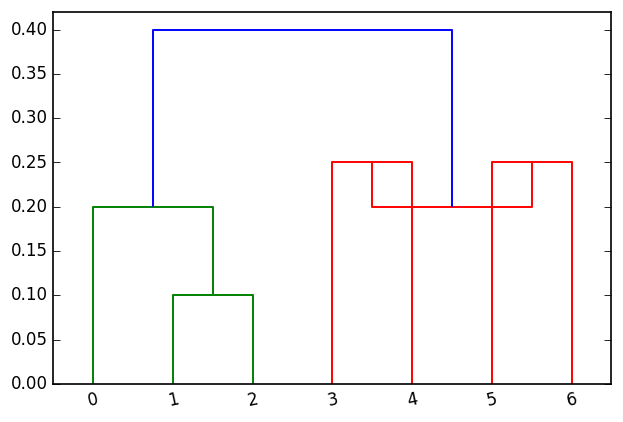
\includegraphics[width=\textwidth]{img/inversion_0.png}
    \caption{\small Dendrograma de inversi\'on.}
     \label{fig:inversion}
\end{minipage} ~
\hfill
\begin{minipage}[b]{0.49\textwidth}
    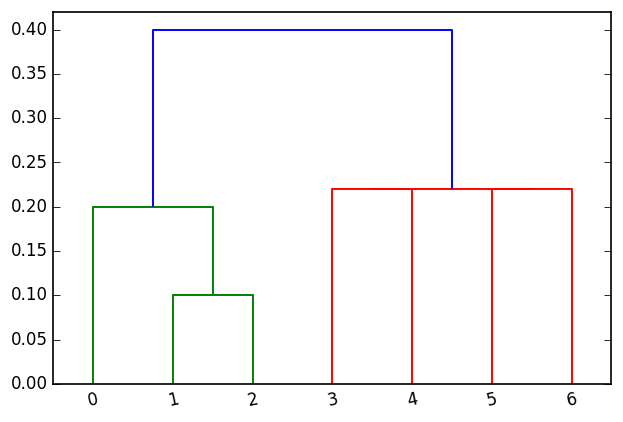
\includegraphics[width=\textwidth]{img/inversion_1.png}
    \caption{\small Dendrograma con inversi\'on corregida. }
    \label{fig:no_inversion}
\end{minipage} ~

\end{figure}  

\vspace{0.1cm}

Otro paso de preprocesamiento es el quitar \textit{outliers} del dendrograma.
Esto en realidad lo hacen durante la etapa de \textit{clustering}. Evitan que los
clusters de un solo elemento se unan a otros clusters si la (di)similitud es 
mayor a cierto \textit{threshold}. Al hacer este paso durante el \textit{clustering}
previenen que los \textit{ouliers} afecten la forma de los nuevos centroides.\\

Una vez finalizados todos los pasos el resultado es un dendrograma. Para parcelar
la corteza solo es necesario seleccionar una altura en la cual cortar dicho
dendrograma. Los clusters que est\'en por debajo de ese corte ser\'an las distintas
parcelas. \\

